\begin{figure}[h] 
\centering 
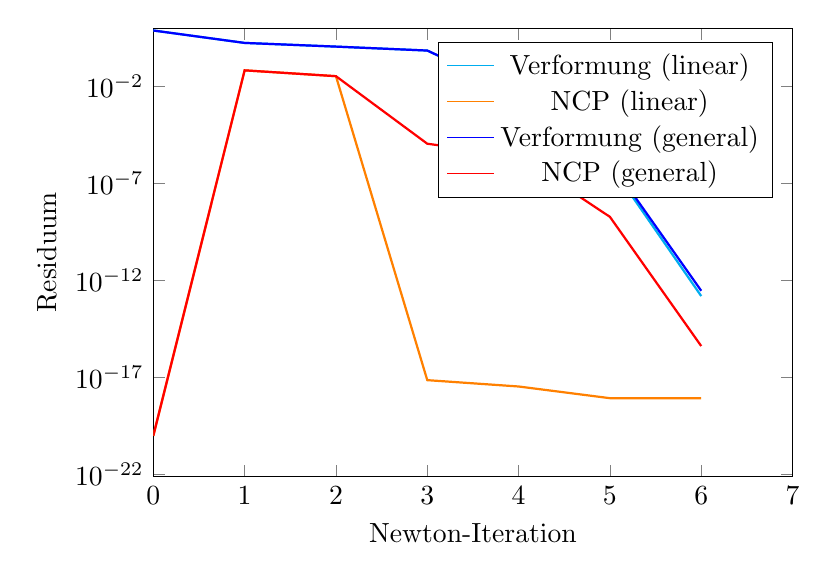
\begin{tikzpicture}[every plot/.append style={thick}] 
\begin{axis}[ 
label style={font=\normalsize}, 
xlabel={Newton-Iteration}, 
ylabel={Residuum}, 
xmin=0, xmax=7, 
ymode=log, 
ymin=0, ymax=10, 
width=0.8\textwidth, 
height=0.6\textwidth, 
legend pos=north east, 
legend style={cells={align=left}}, 
grid style=dashed, 
] 
\addplot[ 
color=cyan, 
] 
coordinates { 
(0, 7.64e+00)(1, 1.75e+00)(2, 1.13e+00)(3, 7.08e-01)(4, 4.61e-03)(5, 9.85e-07)(6, 1.58e-13)}; 
\addlegendentry{Verformung (linear)} 
\addplot[ 
color=orange, 
] 
coordinates { 
(0, 1.00e-20)(1, 6.76e-02)(2, 3.38e-02)(3, 7.37e-18)(4, 3.47e-18)(5, 8.67e-19)(6, 8.67e-19)}; 
\addlegendentry{NCP (linear)} 
\addplot[ 
color=blue, 
] 
coordinates { 
(0, 7.64e+00)(1, 1.75e+00)(2, 1.13e+00)(3, 7.08e-01)(4, 4.80e-03)(5, 1.37e-06)(6, 2.97e-13)}; 
\addlegendentry{Verformung (general)} 
\addplot[ 
color=red, 
] 
coordinates { 
(0, 1.00e-20)(1, 6.76e-02)(2, 3.38e-02)(3, 1.12e-05)(4, 2.56e-06)(5, 1.91e-09)(6, 4.20e-16)}; 
\addlegendentry{NCP (general)} 
\end{axis} 
\end{tikzpicture} 
\caption{Residuen des Stoffgesetzes 'St.Venant' mit Hinderniss 'Parabel' und 18 Freiheitsgraden für die Verschiebung.} 
\label{fiq:St.Venant_Parabel_level0} 
\end{figure} 
